\section*{Глава 2. Проектирование веб-приложения}
\addcontentsline{toc}{section}{Глава 2. Проектирование веб-приложения}
\stepcounter{section}

\subsection{Анализ целевой аудитории}

Разрабатываемое веб-приложение для управления личным гардеробом ориентировано на пользователей, которым необходимо упорядочить информацию о предметах одежды, упростить подбор образов и эффективнее использовать уже имеющиеся вещи. Потребность в таком приложении возникает, когда гардероб становится достаточно разнообразным, а ежедневный выбор одежды требует учета сезона, цвета, типа одежды, стиля, повода и сочетаемости отдельных элементов.

Целевая аудитория приложения включает пользователей, которые регулярно сталкиваются с необходимостью выбора одежды и хотят перенести часть этой задачи в цифровую среду. В отличие от обычного хранения фотографий вещей в галерее телефона, специализированное веб-приложение позволяет структурировать гардероб по категориям, формировать готовые комплекты и повторно использовать их в дальнейшем.

Основную целевую аудиторию можно разделить на несколько пользовательских сегментов:

\begin{itemize}
    \item {Пользователи, стремящиеся к повседневной организации гардероба.} 
    Для них приложение выполняет роль цифрового каталога, где можно хранить информацию о вещах, просматривать их по категориям и формировать базовые повседневные образы. Основная потребность данной группы заключается в снижении времени на выбор одежды.

    \item {Пользователи с большим количеством одежды.} 
    Для данной категории важны функции систематизации гардероба: указание категории, сезона, цвета и типа предмета. Приложение помогает лучше контролировать имеющиеся вещи, избегать повторных покупок и рациональнее использовать гардероб.

    \item {Пользователи, интересующиеся стилем и модой.} 
    Для них приложение является не только инструментом учета одежды, но и средством планирования стиля. Наиболее значимыми функциями являются визуальное представление вещей, возможность комбинировать их между собой и сохранять готовые образы.

    \item {Пользователи, собирающие капсульный гардероб для поездки.} 
    К данной группе относятся пользователи, которым необходимо заранее подобрать ограниченное количество вещей для путешествия, командировки или краткосрочной поездки. Для них важно составить универсальный набор одежды, элементы которого хорошо сочетаются между собой и подходят для разных ситуаций. Приложение помогает заранее спланировать капсулу, избежать лишних вещей в багаже и сделать гардероб для поездки более продуманным и функциональным.

    \item {Пользователи, ориентированные на рациональное потребление.} 
    Цифровой гардероб позволяет лучше понимать, какие вещи уже есть, какие категории перегружены, а каких элементов не хватает. Это способствует снижению импульсивных покупок и более осознанному использованию одежды.
\end{itemize}

Типовые сценарии использования приложения включают добавление нового предмета одежды с указанием названия, категории, цвета и сезона; просмотр гардероба; создание образа из нескольких элементов; сохранение готового комплекта и повторное обращение к нему при необходимости.

Анализ целевой аудитории показывает, что ключевыми требованиями пользователей являются: простое добавление предметов одежды, визуальное представление гардероба, классификация вещей по категориям, цветам и сезонам, удобное формирование и сохранение образов, понятная навигация и доступность приложения через веб-браузер без установки дополнительного программного обеспечения.

Таким образом, целевая аудитория приложения объединена общей потребностью в удобной цифровой организации гардероба. Это определяет основные требования к системе: наглядность, структурированное хранение данных, простоту интерфейса, быстрый доступ к одежде и сохраненным комплектам, а также возможность эффективного планирования повседневных образов.

\subsection{Описание функциональности приложения}

Функциональные возможности разрабатываемого веб-приложения определяются задачами управления личным гардеробом и формирования пользовательских образов.

Основной сценарий использования системы можно представить в виде следующей \textit{User Story}: «Я, как пользователь, хочу добавлять элементы одежды в цифровой гардероб, чтобы хранить информацию о вещах и формировать готовые образы».

На рисунке~\ref{fig:use_case} представлена диаграмма вариантов использования системы.

\begin{figure}[ht!]
	\centering
	
\includegraphics[width=0.5\textwidth]{use_case_diagram}
	\caption{Диаграмма вариантов использования веб-приложения}
	\label{fig:use_case}
\end{figure}

\subsection{Проектирование модели данных}

Для хранения информации в веб-приложении используется реляционная база данных PostgreSQL. База данных проектируется с учетом необходимости хранения данных о пользователях, категориях одежды, элементах гардероба и сформированных пользовательских образах.

Структура базы данных включает 5 таблиц:
\begin{itemize}
	\item \texttt{users} --- хранение учетных записей пользователей;
	\item \texttt{categories} --- хранение категорий одежды;
	\item \texttt{clothes} --- хранение элементов гардероба;
	\item \texttt{outfits} --- хранение пользовательских образов;
	\item \texttt{outfit\_items} --- связь между образами и элементами одежды.
\end{itemize}

Связь между пользователями и элементами одежды имеет тип «один ко многим», так как один пользователь может добавить несколько предметов гардероба. Связь между пользователями и образами также имеет тип «один ко многим», поскольку один пользователь может создать несколько образов. Связь между образами и элементами одежды реализуется через промежуточную таблицу, так как один образ может содержать несколько предметов одежды, а один предмет одежды может использоваться в разных образах.

Структура таблицы пользователей представлена в табл.~\ref{tab:db_users}.

\begin{longtable}{|l|l|p{3.5cm}|p{5.5cm}|}
	\caption{Структура таблицы пользователей (\texttt{users})}
	\label{tab:db_users} \\

	\hline
	\textbf{Поле} & \textbf{Тип} & \textbf{Ограничение} & \textbf{Описание} \\ \hline
	\endfirsthead

	\tabcont{\ref{tab:db_users}}
	\textbf{Поле} & \textbf{Тип} & \textbf{Ограничение} & \textbf{Описание} \\ \hline
	\endhead

	\hline
	\endfoot

	\hline
	\endlastfoot

	id & SERIAL & PRIMARY KEY & Уникальный идентификатор пользователя \\ \hline
	username & VARCHAR(50) & NOT NULL & Имя пользователя в системе \\ \hline
	email & VARCHAR(100) & UNIQUE, NOT NULL & Электронная почта пользователя \\ \hline
	password\_hash & VARCHAR(255) & NOT NULL & Хеш пароля пользователя \\ \hline
	role & VARCHAR(20) & DEFAULT 'user', NOT NULL & Роль пользователя в системе \\ \hline
\end{longtable}

Таблица \texttt{users} предназначена для хранения учетных записей пользователей. Поле \texttt{email} является уникальным, что исключает регистрацию нескольких пользователей с одинаковой электронной почтой. Пароль хранится не в открытом виде, а в виде хеша. Поле \texttt{role} используется для разграничения прав доступа. Значение \texttt{user} соответствует обычному пользователю, а значение \texttt{admin} --- администратору.

Структура таблицы категорий представлена в табл.~\ref{tab:db_categories}.

\begin{longtable}{|l|l|p{3.5cm}|p{5.5cm}|}
	\caption{Структура таблицы категорий одежды (\texttt{categories})}
	\label{tab:db_categories} \\

	\hline
	\textbf{Поле} & \textbf{Тип} & \textbf{Ограничение} & \textbf{Описание} \\ \hline
	\endfirsthead

	\tabcont{\ref{tab:db_categories}}
	\textbf{Поле} & \textbf{Тип} & \textbf{Ограничение} & \textbf{Описание} \\ \hline
	\endhead

	\hline
	\endfoot

	\hline
	\endlastfoot

	id & SERIAL & PRIMARY KEY & Уникальный идентификатор категории \\ \hline
	name & VARCHAR(50) & UNIQUE, NOT NULL & Название категории одежды \\ \hline
\end{longtable}

Таблица \texttt{categories} используется для классификации элементов гардероба. Категория описывает общий тип одежды, например: верхняя одежда, обувь, брюки, футболки или аксессуары. Отдельная таблица категорий позволяет избежать дублирования одинаковых названий категорий в таблице одежды.

Структура таблицы одежды представлена в табл.~\ref{tab:db_clothes}.

\begin{longtable}{|l|l|p{3.5cm}|p{5.5cm}|}
	\caption{Структура таблицы одежды (\texttt{clothes})}
	\label{tab:db_clothes} \\

	\hline
	\textbf{Поле} & \textbf{Тип} & \textbf{Ограничение} & \textbf{Описание} \\ \hline
	\endfirsthead

	\tabcont{\ref{tab:db_clothes}}
	\textbf{Поле} & \textbf{Тип} & \textbf{Ограничение} & \textbf{Описание} \\ \hline
	\endhead

	\hline
	\endfoot

	\hline
	\endlastfoot

	id & SERIAL & PRIMARY KEY & Уникальный идентификатор элемента одежды \\ \hline
	user\_id & INTEGER & FOREIGN KEY, NOT NULL & Ссылка на пользователя \\ \hline
	category\_id & INTEGER & FOREIGN KEY, NOT NULL & Ссылка на категорию одежды \\ \hline
	name & VARCHAR(100) & NOT NULL & Название предмета одежды \\ \hline
	color & VARCHAR(50) & NULL & Цвет элемента одежды \\ \hline
	season & VARCHAR(20) & NULL & Сезон использования \\ \hline
	image\_path & TEXT & NOT NULL & Путь к изображению одежды \\ \hline
\end{longtable}

Таблица \texttt{clothes} является основной таблицей для хранения предметов гардероба. Каждый элемент одежды принадлежит конкретному пользователю и относится к определенной категории. Поле \texttt{image\_path} хранит путь к изображению предмета одежды, которое отображается в интерфейсе приложения.

Структура таблицы образов представлена в табл.~\ref{tab:db_outfits}.

\begin{longtable}{|l|l|p{3.5cm}|p{5.5cm}|}
	\caption{Структура таблицы образов (\texttt{outfits})}
	\label{tab:db_outfits} \\

	\hline
	\textbf{Поле} & \textbf{Тип} & \textbf{Ограничение} & \textbf{Описание} \\ \hline
	\endfirsthead

	\tabcont{\ref{tab:db_outfits}}
	\textbf{Поле} & \textbf{Тип} & \textbf{Ограничение} & \textbf{Описание} \\ \hline
	\endhead

	\hline
	\endfoot

	\hline
	\endlastfoot

	id & SERIAL & PRIMARY KEY & Уникальный идентификатор образа \\ \hline
	user\_id & INTEGER & FOREIGN KEY, NOT NULL & Ссылка на пользователя \\ \hline
	name & VARCHAR(100) & NOT NULL & Название образа \\ \hline
\end{longtable}

Таблица \texttt{outfits} предназначена для хранения пользовательских образов. Каждый образ принадлежит конкретному пользователю и представляет собой комплект одежды, составленный из добавленных элементов гардероба.

Структура таблицы связи образов и элементов одежды представлена в табл.~\ref{tab:db_outfit_items}.

\begin{longtable}{|l|l|p{3.5cm}|p{5.5cm}|}
	\caption{Структура таблицы элементов образа (\texttt{outfit\_items})}
	\label{tab:db_outfit_items} \\

	\hline
	\textbf{Поле} & \textbf{Тип} & \textbf{Ограничение} & \textbf{Описание} \\ \hline
	\endfirsthead

	\tabcont{\ref{tab:db_outfit_items}}
	\textbf{Поле} & \textbf{Тип} & \textbf{Ограничение} & \textbf{Описание} \\ \hline
	\endhead

	\hline
	\endfoot

	\hline
	\endlastfoot

	outfit\_id & INTEGER & PRIMARY KEY, FOREIGN KEY & Ссылка на образ \\ \hline
	clothes\_id & INTEGER & PRIMARY KEY, FOREIGN KEY & Ссылка на элемент одежды \\ \hline
\end{longtable}

Таблица \texttt{outfit\_items} является промежуточной таблицей и реализует связь «многие ко многим» между таблицами \texttt{outfits} и \texttt{clothes}. Благодаря такой структуре один образ может включать несколько предметов одежды, а один и тот же предмет одежды может использоваться в разных образах.

Разработанная структура базы данных включает только необходимые для учебного проекта таблицы: пользователей, категории, элементы одежды, образы и элементы образов. 
Такая модель позволяет хранить данные личного гардероба, связывать вещи с пользователями и категориями, а также формировать образы из нескольких предметов одежды. 

На рисунке~\ref{fig:er_diagram} представлена ER-диаграмма базы данных.

\begin{figure}[ht!]
	\centering
	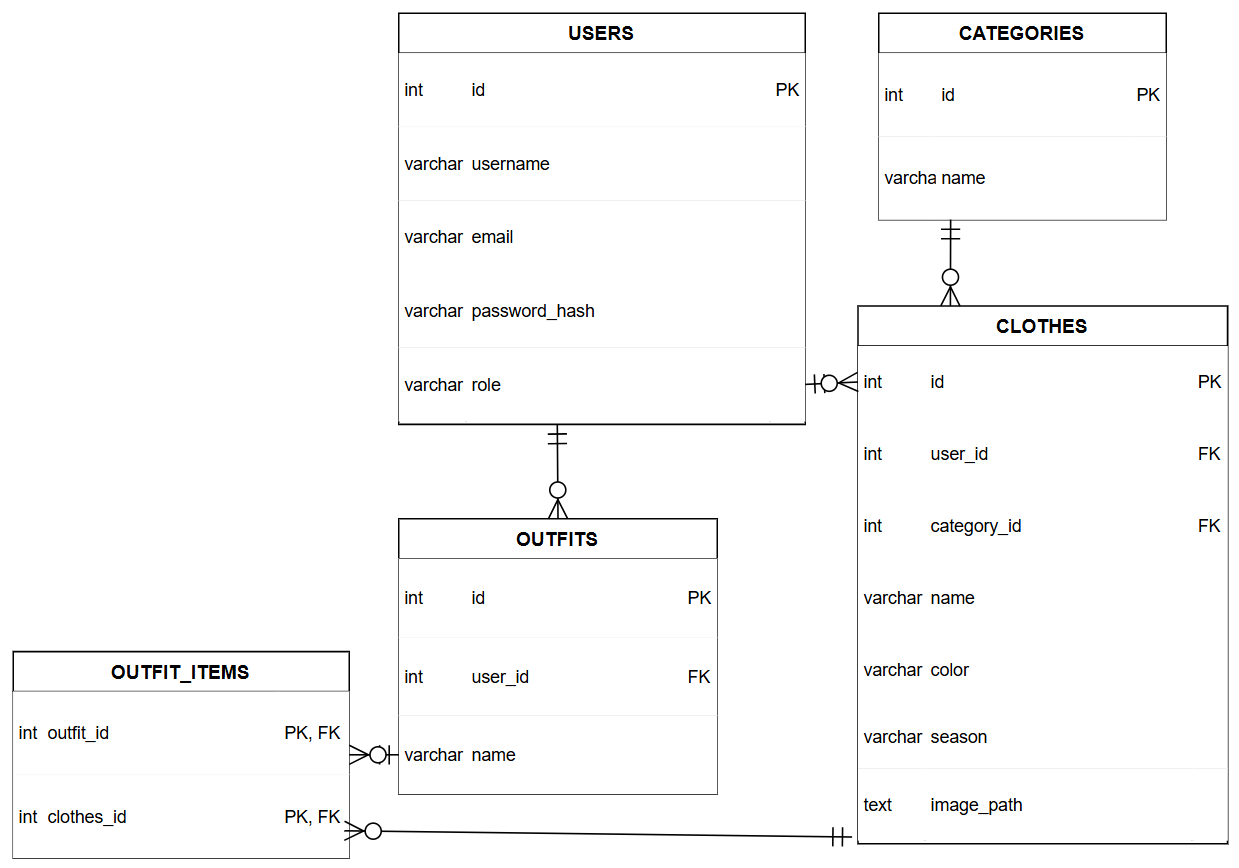
\includegraphics[width=0.75\textwidth]{images/er_diagram.png}
	\caption{ER-диаграмма базы данных}
	\label{fig:er_diagram}
\end{figure}


\subsection{Разработка макетов страниц}

На этапе проектирования интерфейса были разработаны макеты основных страниц веб-приложения. При создании интерфейса учитывались требования к удобству использования, простоте навигации и наглядному отображению элементов гардероба.

На рисунке~\ref{fig:login-page} представлен макет страницы авторизации пользователя. Данная страница предназначена для входа зарегистрированного пользователя в систему.

\begin{figure}[ht!]
	\centering
	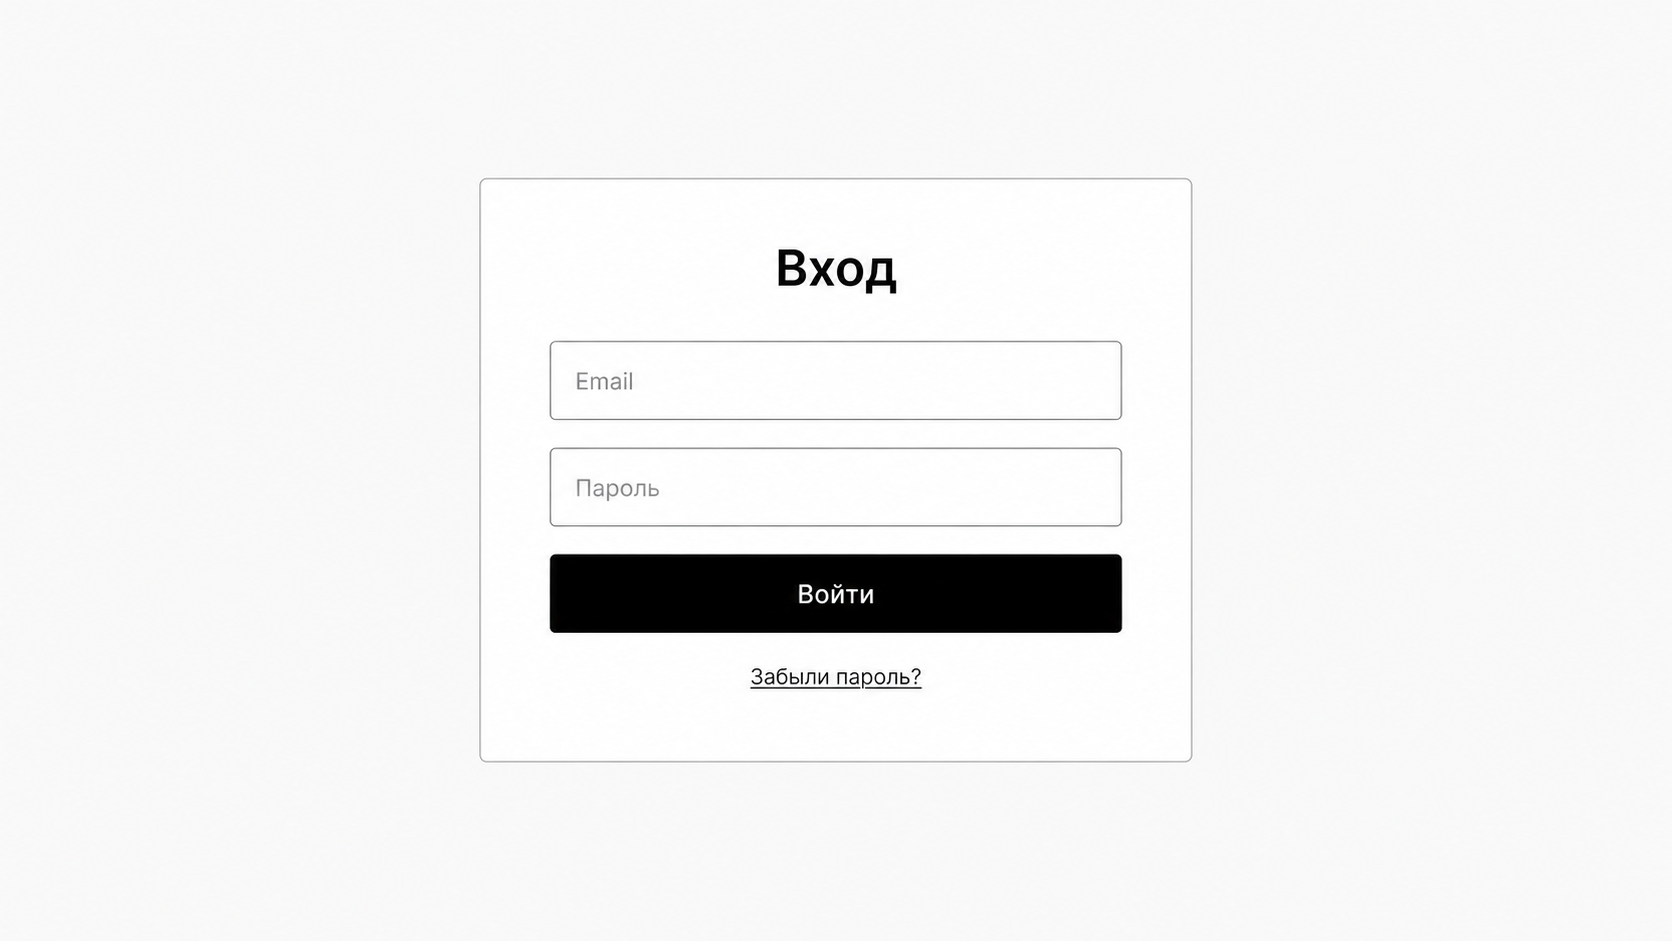
\includegraphics[width=0.9\textwidth]{images/templates/login.png}
	\caption{Макет страницы авторизации пользователя}
	\label{fig:login-page}
\end{figure}

На рисунке~\ref{fig:registration-page} представлен макет страницы регистрации пользователя. На данной странице пользователь может создать новую учетную запись для дальнейшей работы с приложением.

\begin{figure}[ht!]
	\centering
	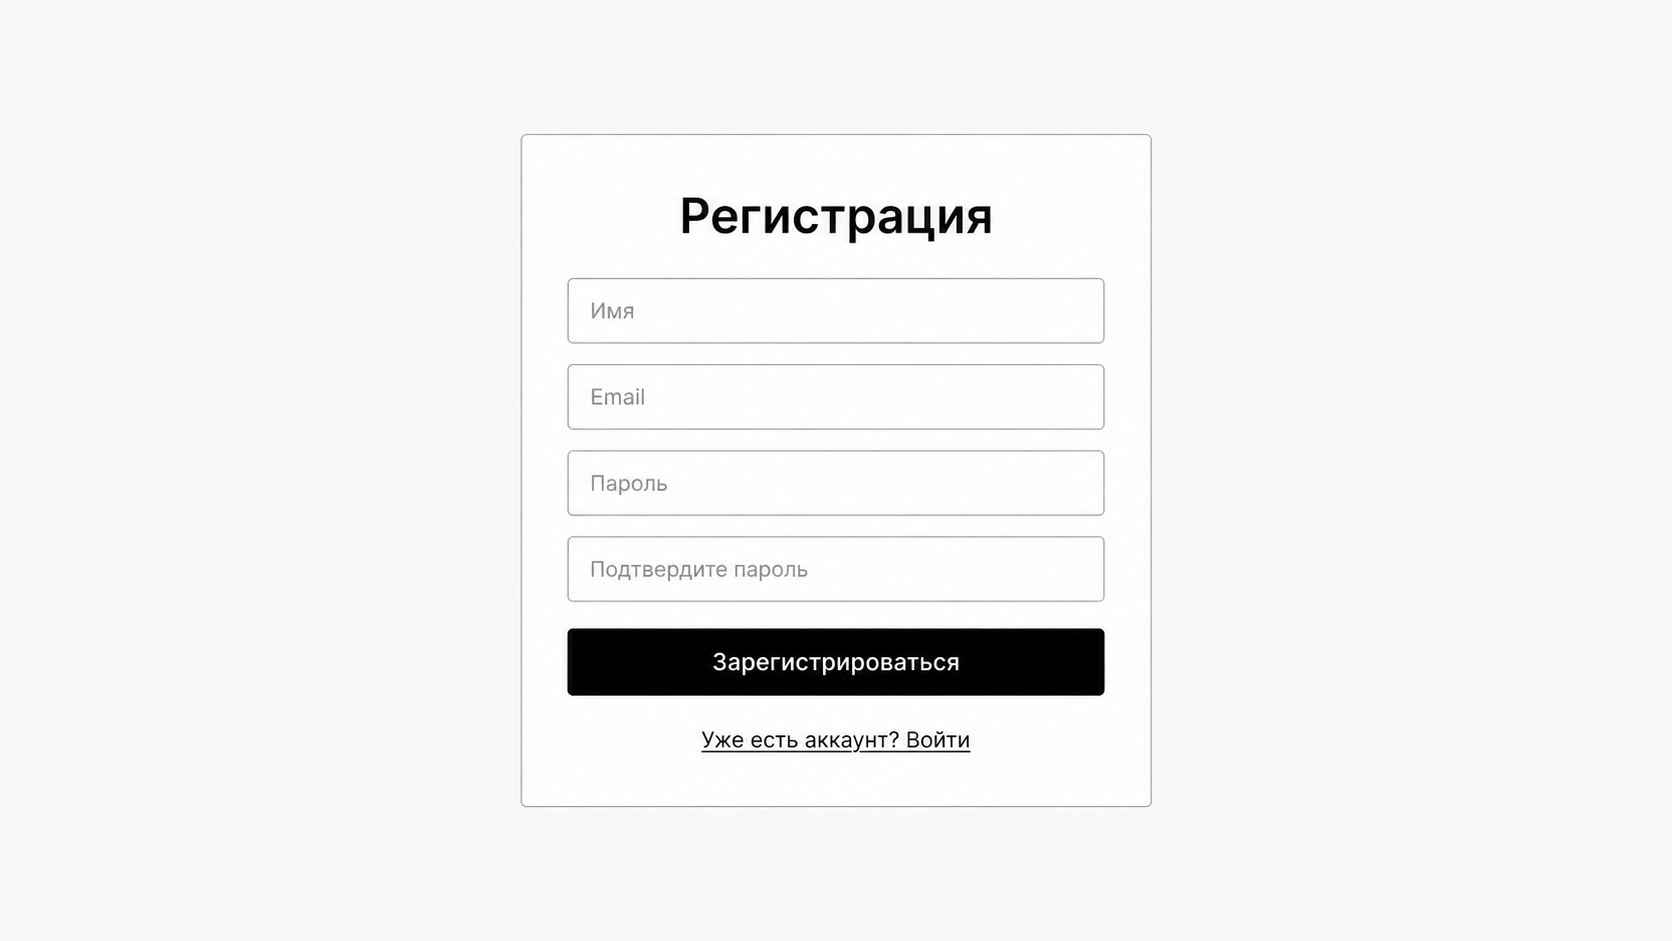
\includegraphics[width=0.9\textwidth]{images/templates/registration.png}
	\caption{Макет страницы регистрации пользователя}
	\label{fig:registration-page}
\end{figure}

На рисунке~\ref{fig:main-page} представлен макет главной страницы со списком элементов гардероба. Страница позволяет просматривать добавленные предметы одежды, выполнять поиск, фильтрацию, редактирование и удаление записей.

\begin{figure}[ht!]
	\centering
	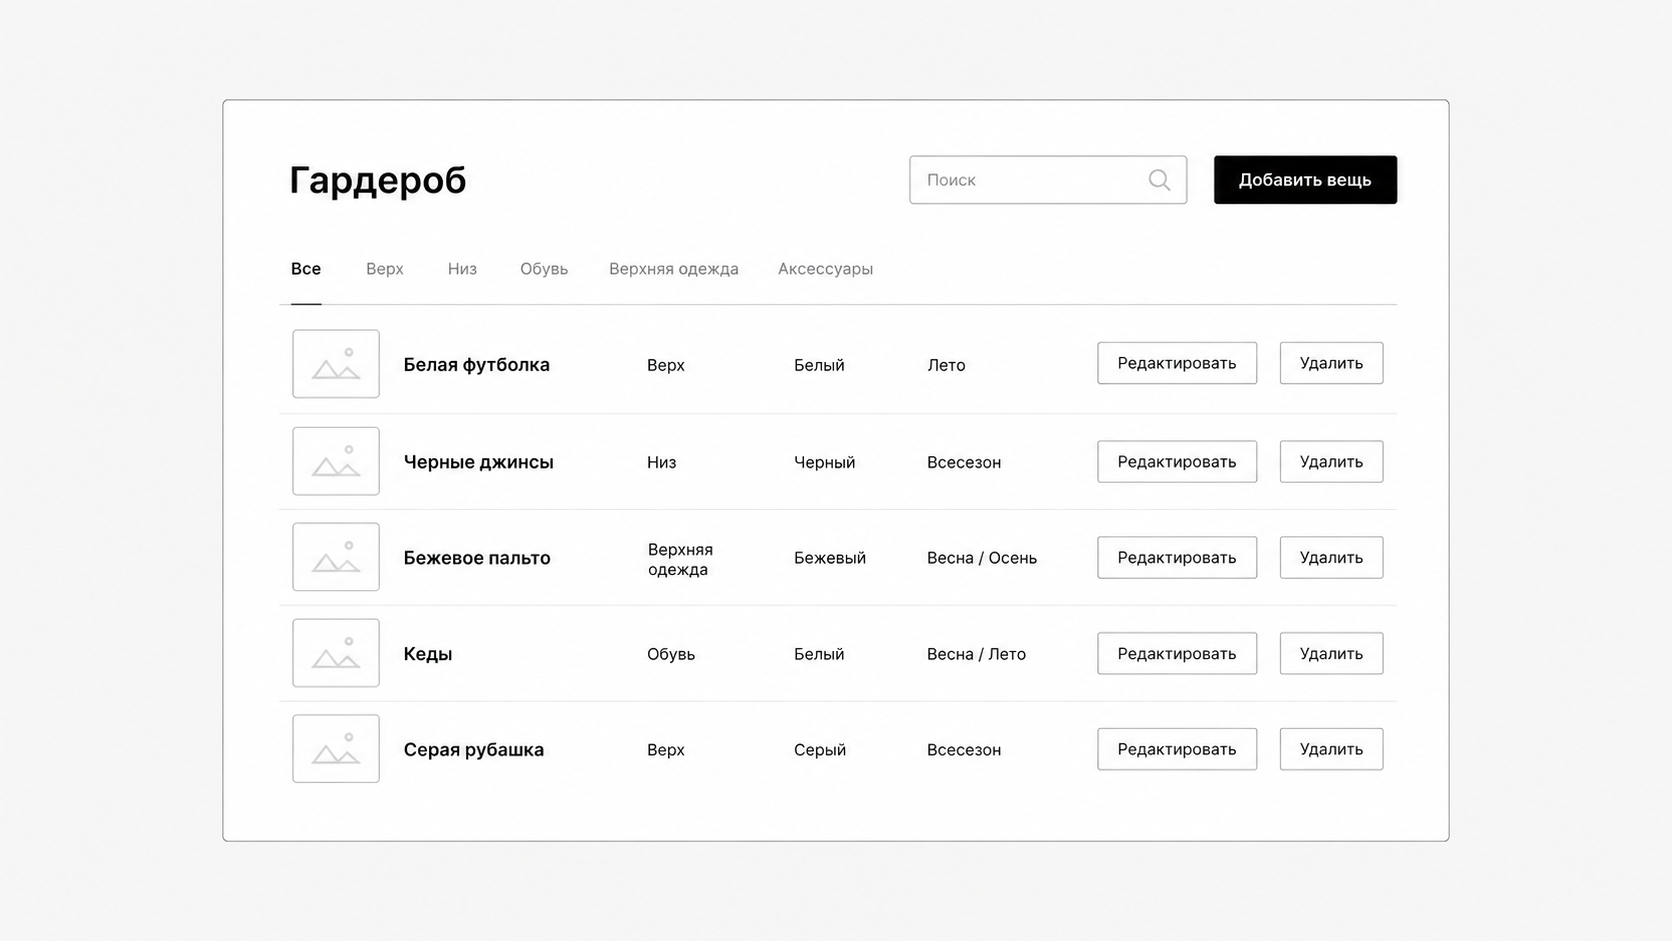
\includegraphics[width=0.9\textwidth]{images/templates/main-page.png}
	\caption{Макет главной страницы со списком элементов гардероба}
	\label{fig:main-page}
\end{figure}

На рисунке~\ref{fig:adding-clothes-page} представлен макет страницы добавления новой одежды. Данная страница содержит форму для загрузки изображения предмета одежды и заполнения основной информации о нем.

\begin{figure}[ht!]
	\centering
	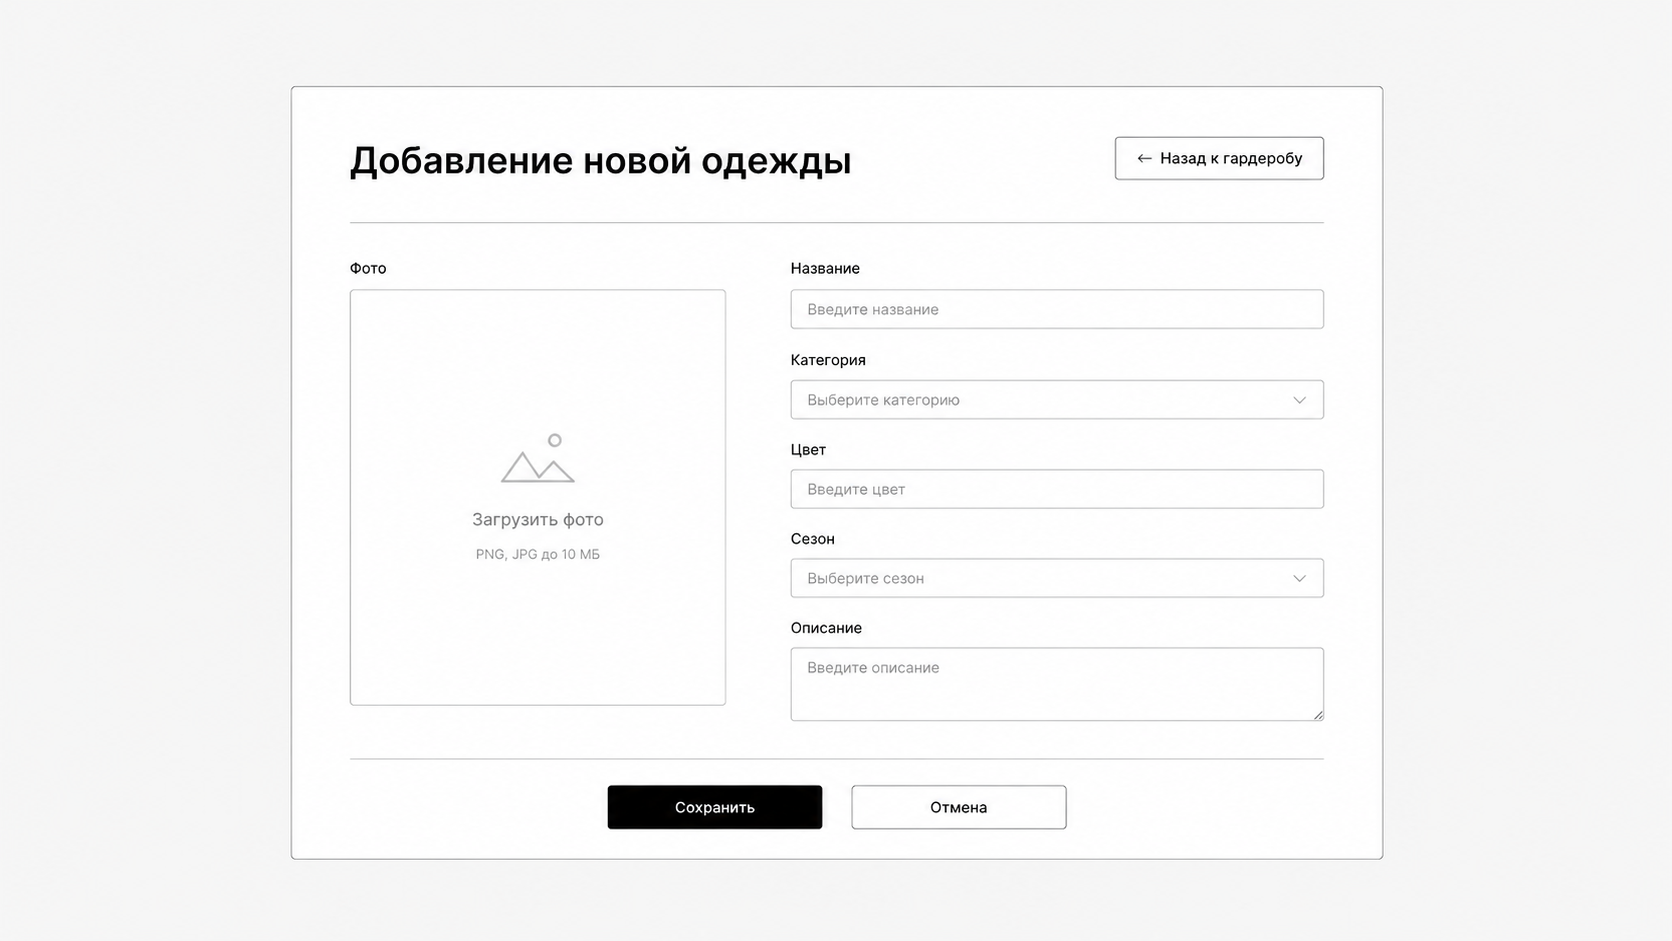
\includegraphics[width=0.9\textwidth]{images/templates/adding-clothes.png}
	\caption{Макет страницы добавления новой одежды}
	\label{fig:adding-clothes-page}
\end{figure}

На рисунке~\ref{fig:viewing-and-editing-page} представлен макет страницы просмотра и редактирования информации о предмете одежды. На данной странице пользователь может изменить данные выбранного элемента гардероба или удалить его из системы.

\begin{figure}[ht!]
	\centering
	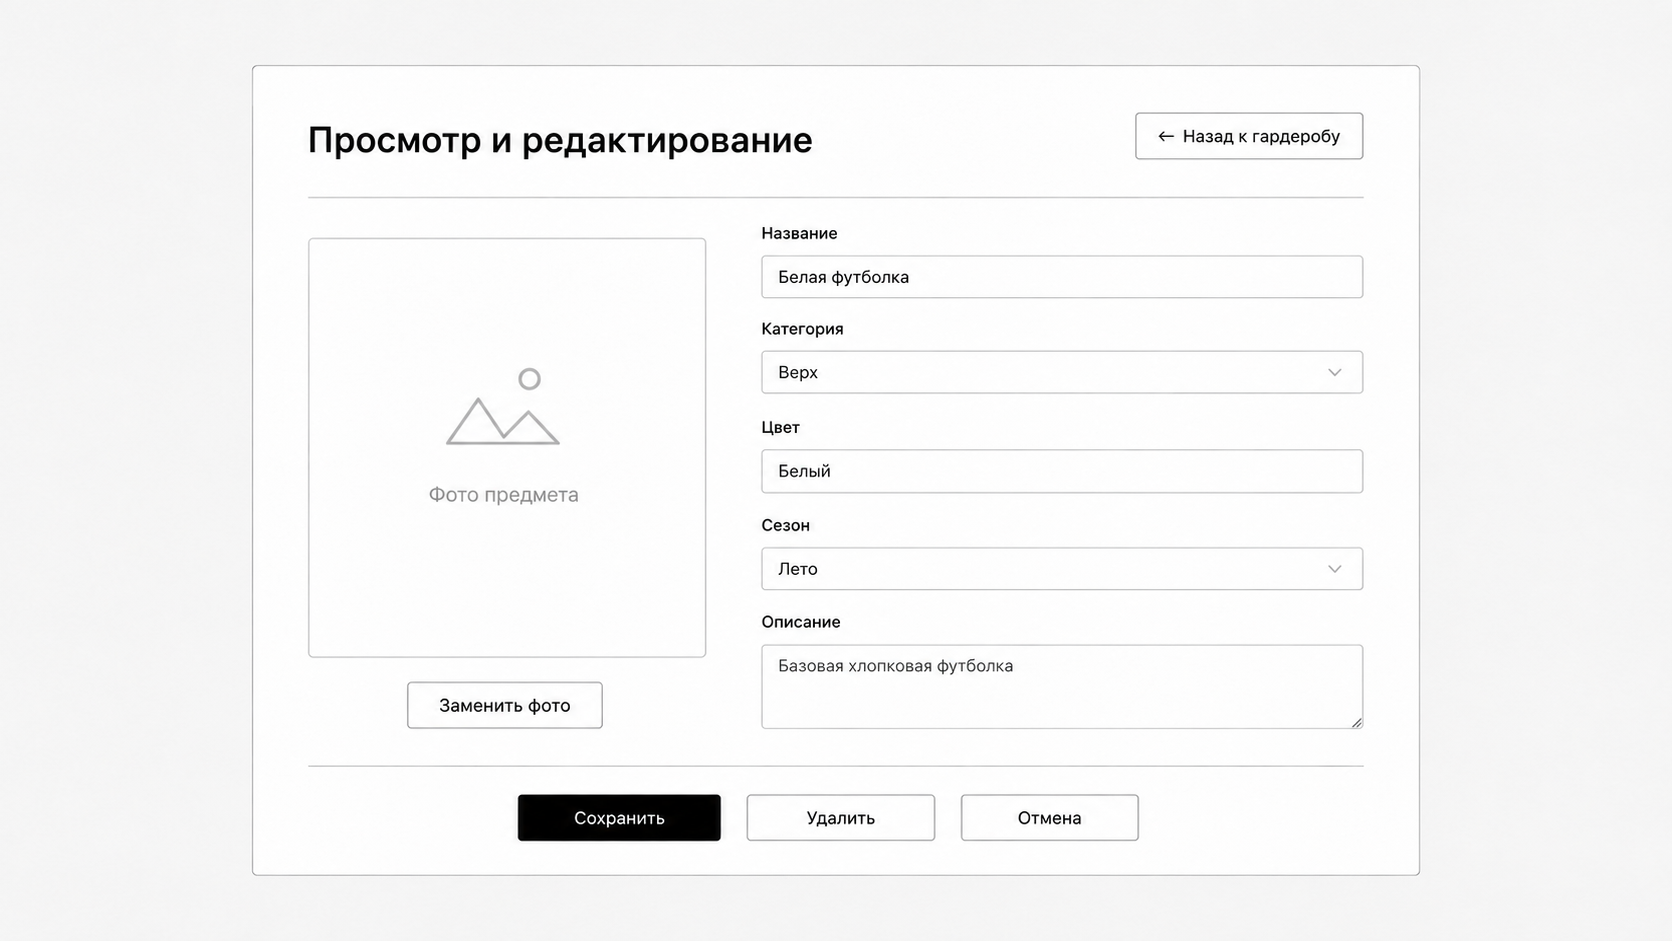
\includegraphics[width=0.9\textwidth]{images/templates/viewing-and-editing.png}
	\caption{Макет страницы просмотра и редактирования информации о предмете одежды}
	\label{fig:viewing-and-editing-page}
\end{figure}

На рисунке~\ref{fig:creating-images-page} представлен макет страницы создания пользовательских образов. Страница позволяет выбрать элементы гардероба, добавить их в состав образа и сохранить готовый комплект одежды.

\begin{figure}[ht!]
	\centering
	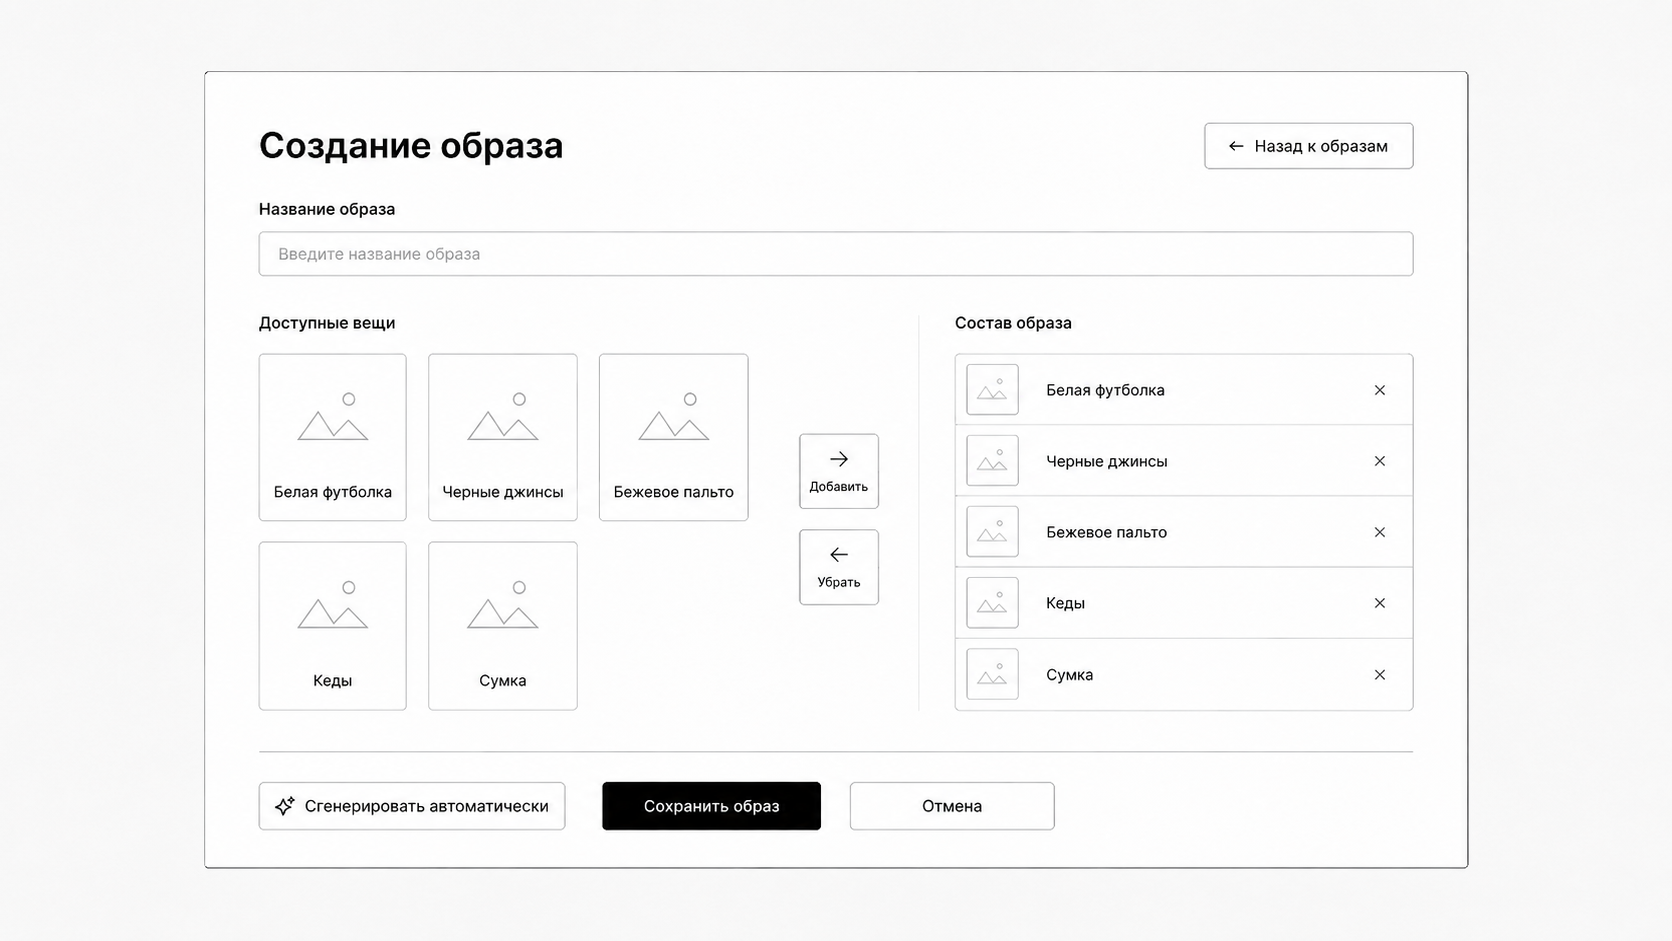
\includegraphics[width=0.9\textwidth]{images/templates/creating-images.png}
	\caption{Макет страницы создания пользовательских образов}
	\label{fig:creating-images-page}
\end{figure}

На рисунке~\ref{fig:saved-images-page} представлен макет страницы просмотра сохранённых комплектов одежды. Данная страница предназначена для просмотра ранее созданных образов, их редактирования и удаления.

\begin{figure}[ht!]
	\centering
	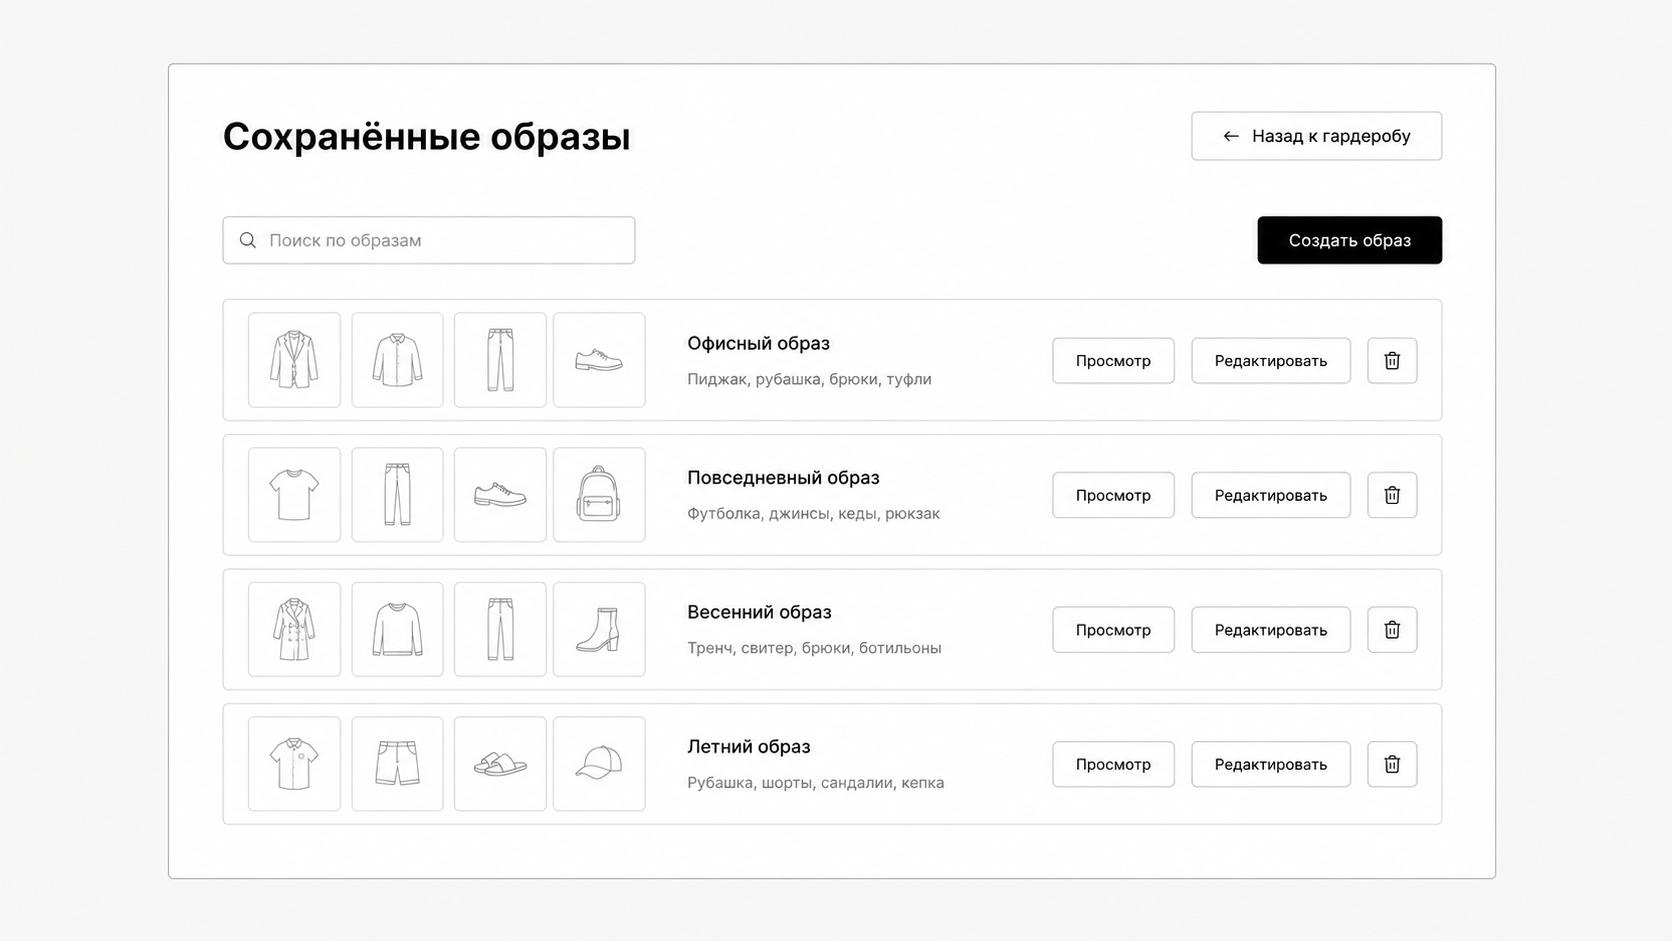
\includegraphics[width=0.9\textwidth]{images/templates/saved-images.png}
	\caption{Макет страницы просмотра сохранённых комплектов одежды}
	\label{fig:saved-images-page}
\end{figure}